\section{Navigation}\label{sec:navigation}
As mention in the previous Section we use of the navigation drawer in our application, the navigation drawer is a navigation design pattern acknowledged and used by Google.\cite{guidelines-navigationdrawer} The navigation drawer is the central widget for navigation in our application.
 
\subsection{Navigation drawer}
The navigation drawer is a powerful design that allows the user from any views in the application to navigate to top level views. The navigation drawer is expanded from the left of the application.
\begin{figure}[H]
\centering
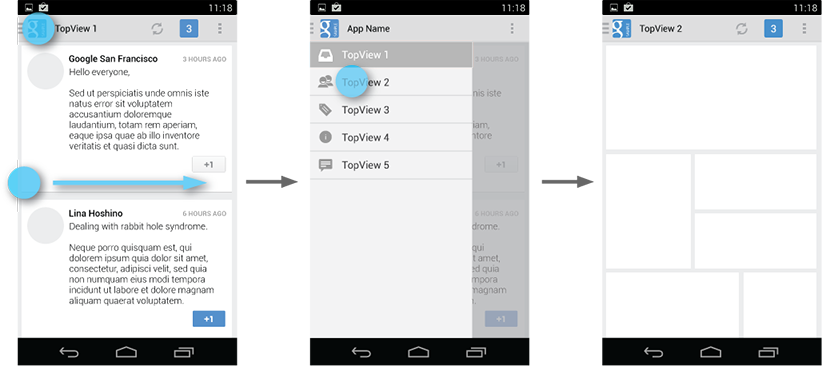
\includegraphics[width=0.9\linewidth]{img/screenshots/navigation_drawer_overview.png}
\caption{Navigation drawer overview \cite{guidelines-navigationdrawer}}
\label{fig:navigationdrawer}
\end{figure}
There are two different ways of expanding the navigation drawer, the consistent one being swiping from the left edge of the screen to the centre, this can always be achieved no matter the context. 
The second one being pressing the button in the top left corner, the button the marked with three lines, The \autoref{fig:navigationdrawer} illustrates this. 
The reason for the second option not being consistent is if the user navigates to a lower view the button transforms to a return button, if pressed this return button will navigate the user to the top most view. 
Each item in the navigation drawer navigates to different top-level pages in the application or typical main actions like sign in/sign out.

\subsection{Application navigation}
Our application has six top level views; ingredient search, recipe search, favourites, shopping list\todo{Should we still write "shopping list" even if we did not implement it}, settings, sign in/sign out. 
We only have one lower level view in our application which is a recipe. Some views in the application might require the user to be signed in, for them to be available. 
Like the view favourites, which displays the recipes that the user has favourited. 
If the user is not signed in when trying to enter the favourite view, they are met a text asking them to sign in.
\todo{Show an example with pictures}
